\subsection{A Deeper U-Net Mala}

The first network we implemented is a U-Net Mala with a deeper architecture using zero padding for every convolution operation. We tried this experience because a deeper architecture is often associated with deeper meaning representation during learning. A padding for every convolution allows us to stack more layers adding a 5th level with 1024 filters without diminishing the size of the output gradient predictions along height and width.
As previous experiences, the network takes a $256\times256$ input image and output the gradients along $x$ and $y$ axes for the whole image. Convolutional layers with $3\times3$ kernel size and Rectified Linear Unit activations are also used and max pooling operations stay the same.
Bilinear upsampling layers are replaced by transposed convolutions as described in \cite{funke_large_2019}.\\

The network is trained for 230.000 iterations using an Adam optimizer with an initial learning rate $\alpha = 10^{-4}$, $\beta_{1}=0.95$, $\beta_{2}=0.99$ et $\epsilon=10^{-8}$. During inference,  a simple pixel wise mean followed by a threshold is applied to the two gradient volumes to create the final segmentation.\\

With this network, we were able to generate thinner segmentations for every frame and get better results on the Cremi test-set than previous experiences.


\subsection{Multi Input Images}

This architecture came with the idea to use 3 successive frames as input and compute the loss only on the center image in order to predict a better segmentation along the depth. As we know, Cremi is a volume dataset so a network linking a frame to its neighbors should better predict segmentations along the depth than previous networks.\\
This network shares the same architecture as U-Net Mala described in previous works, optimizer and other hyperparameters for training and inference remain the same.\\

\subsection{3D U-Net Mala}

One of our main objective was to implement the network as described in \cite{funke_large_2019}. This part describes the implementation of a 3 dimensional U-Net like architecture for volume segmentation. Mathematical operations and training parameters are the same as described in the paper. The network takes $84\times268\times268$ (depth, height, width) patches as input and predict the gradient along x, y and z axes defined by $56\times56\times56$ outputs.\\

\begin{figure}[!htbp]
	\centering
	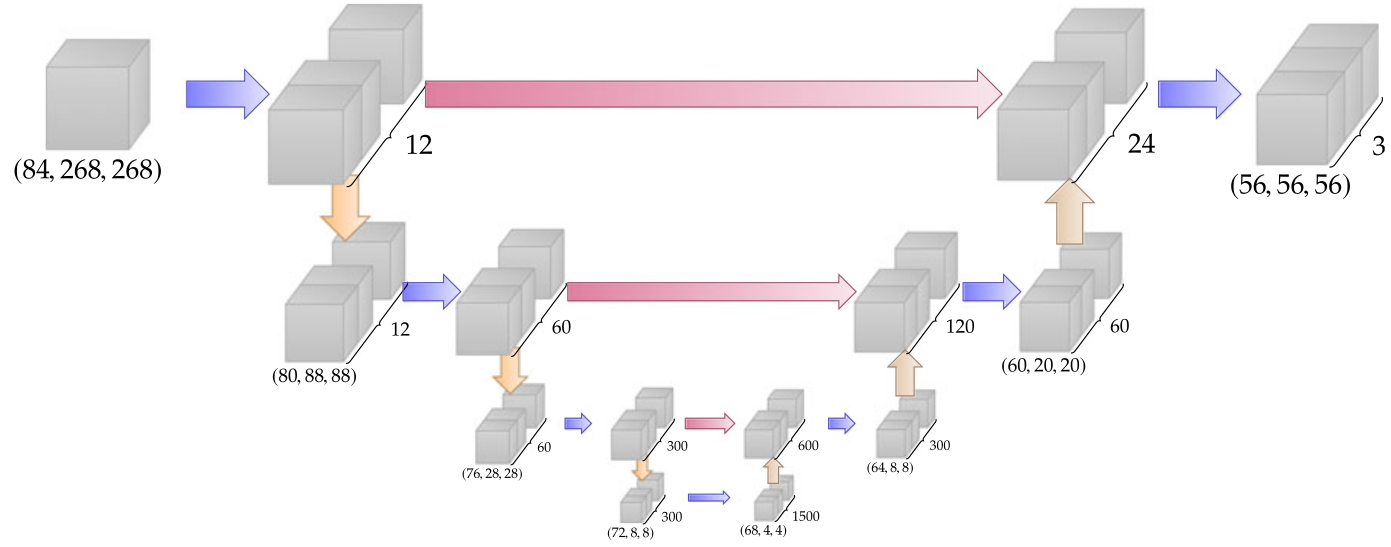
\includegraphics[width=0.8\linewidth]{./images/mala_architecture.png}
	\caption{Overview of the U-Net architecture used for the Cremi dataset in \cite{funke_large_2019}. The network is 4 levels deep and doesn’t use padding for convolution operations. Transposed convolutions and max pooling layers use a stride of 3 along height and width but do not affect the input size along the depth. Relu activations are used after every convolution layer.}%
	\label{fig:mala_unet}
\end{figure}

To implement the network, we created a 3D version of the processing algorithms for calculating edge weights and decompose the dataset into patches. For inference, every patch of the volume is fed into the network, then gradients volumes are reconstructed for the 3 axes.

\begin{figure}[!htbp]
	\centering
	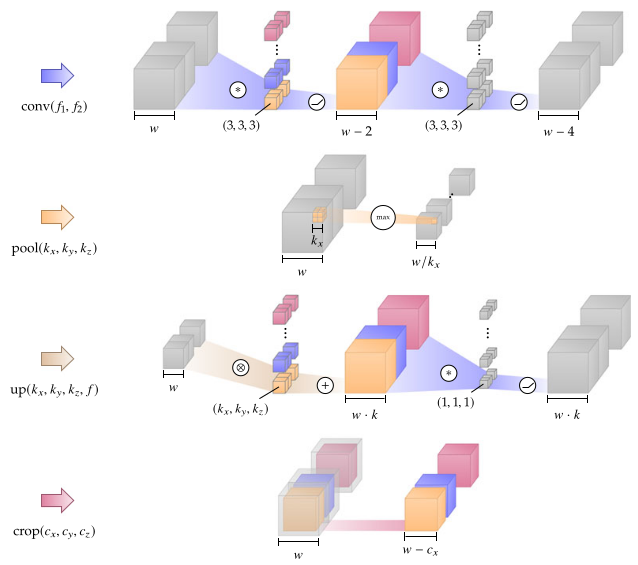
\includegraphics[width=0.8\linewidth]{./images/architecture_details.png}
	\caption{Details of convolution operations (blue), pooling (orange), transpose convolution (brown) and crops (red). Every transpose convolution layer is followed by a concatenation operation between outputs and crops from the same level.  A $1\times1\times1$ convolution follows the concatenation to reduce the filter dimension.}%
	\label{fig:mala_unet}
\end{figure}


